% !TEX root = hw10-answers.tex
\chead{\textbf{Exercises week 10}}
\begin{document}
\flushleft\textbf{Topic: Structural Causal Models and Graphs}
% \section{In linear SCMs, solvability follow from invertibility}
% We call an SCM $\C{M}=\langle \Sin, \Send, \Srnd, \CX, P, f \rangle$
% \emph{linear} if all variables are real-valued and 
% each component of the causal mechanism is a linear combination of variables, that is
% $$
%   f_v(x) = \sum_{w\in V \cup J \cup W} B_{vw} x_w,
% $$
% where $B\in\RN^{V \times (V \cup J \cup W)}$ is a matrix of coefficients.

% \begin{enumerate}
% \item Show that for any set $L \subseteq V$, $(\C{M})_{\doit(V\setminus L)}$ is uniquely solvable if and only if the matrix $I_{L}-B_{LL}$ is invertible. Give the unique solutions function. (1pt)
% \item Bonus: generalize and prove this statement for non-linear SCMs and invertible non-linear functions. (1pt)
% \end{enumerate}

\section{Graphs of SCMs and marginals}
Given SCM: $\C M = \left\langle J=\emptyset, V=\{A, B, C, D\}, W=\{\epsilon_A, \epsilon_B, \epsilon_C, \epsilon_D\}, \R^8, P, f \right\rangle$, where $P$ are four independent normal distributions with means and standard deviations $\mu_A, \sigma_A, \mu_B, \sigma_B$ etc. and:
\[
\begin{pmatrix}
	f_A(x) \\ f_B(x) \\ f_C(x) \\ f_D(x)
\end{pmatrix}
= 
\begin{pmatrix}
	0 & 0 & 0 & 0 \\
	\alpha_{ab} & 0 & 0 & \alpha_{db} \\
	0 & \alpha_{bc} & 0 & \alpha_{dc} \\
	\alpha_{ad} & 0 & 0 & 0 \\
\end{pmatrix}
\begin{pmatrix}
	A \\ B \\ C \\ D
\end{pmatrix}
+
\begin{pmatrix}
	\epsilon_A \\ \epsilon_B \\ \epsilon_C \\ \epsilon_D
\end{pmatrix}
\]
for nonzero real numbers $\alpha_.$. Note that we are abusing notation and refer to $A$ as both a node and variable $A \in \R$.
\begin{enumerate}
	\item Construct a solution function. (1/2pt)
\begin{gradedsolution}
	As the SCM is acyclic with order e.g. $(A,D,B,C)$, the solution can be read off from $f$. Alternatively, use  $(1_4-B_{VV})^{-1}\epsilon$.
	One finds:
	\[
	\mat{
		\text{A} \leftarrow \epsilon _A \\
		\text{B} \leftarrow \epsilon _A \left(\alpha _{\text{ab}}+\alpha _{\text{ad}} \alpha _{\text{db}}\right)+\epsilon _B+\epsilon _D \alpha _{\text{db}} \\
		\text{C} \leftarrow \epsilon _A \left(\alpha _{\text{ab}} \alpha _{\text{bc}}+\alpha _{\text{ad}} \alpha _{\text{bc}} \alpha _{\text{db}}+\alpha _{\text{ad}} \alpha _{\text{dc}}\right)+\epsilon _B \alpha _{\text{bc}}+\epsilon _D \left(\alpha _{\text{bc}} \alpha _{\text{db}}+\alpha _{\text{dc}}\right)+\epsilon _C \\
		\text{D} \leftarrow \epsilon _A \alpha _{\text{ad}}+\epsilon _D
	}
	\]

\end{gradedsolution}
	\item Give the graph $G(\C M)$. (1/2pt)
	\begin{gradedsolution}
	\begin{tikzpicture}[scale=1, transform shape]
		\tikzstyle{every node} = [draw,shape=circle];
		\node (A) at (0, 2) {$A$};
		\node (B) at (1, 0) {$B$};
		\node (C) at (3, 0) {$C$};
		\node (D) at (2, 2) {$D$};
		\node (epsA) at (0, 4) {$\epsilon_A$};
		\node (epsB) at (1, -2) {$\epsilon_B$};
		\node (epsC) at (3, -2) {$\epsilon_C$};
		\node (epsD) at (2, 4) {$\epsilon_D$};
		\draw[-{Latex[length=3mm, width=2mm]}] (A) to (B);
		\draw[-{Latex[length=3mm, width=2mm]}] (A) to (D);
		\draw[-{Latex[length=3mm, width=2mm]}] (D) to (C);
		\draw[-{Latex[length=3mm, width=2mm]}] (D) to (B);
		\draw[-{Latex[length=3mm, width=2mm]}] (B) to (C);
		\draw[-{Latex[length=3mm, width=2mm]}] (epsA) to (A);
		\draw[-{Latex[length=3mm, width=2mm]}] (epsB) to (B);
		\draw[-{Latex[length=3mm, width=2mm]}] (epsC) to (C);
		\draw[-{Latex[length=3mm, width=2mm]}] (epsD) to (D);
	\end{tikzpicture}
		
	\end{gradedsolution}
	\item For latents $L=\{D\}$, give the marginal SCM $\C M_{\setminus L}$ and its solution. (1pt)
\begin{gradedsolution}
	Intervening on $\{A,B,C\}$, we solve for $D$ and find $D=\alpha_{ad} A + \epsilon_D$. Filling this in leads to:
	\begin{align*}
	\begin{pmatrix}
		f_A(x) \\ f_B(x) \\ f_C(x)
	\end{pmatrix}
	&= 
	\begin{pmatrix}
		0 & 0 & 0 & 0 \\
		\alpha_{ab} & 0 & 0 & \alpha_{db} \\
		0 & \alpha_{bc} & 0 & \alpha_{dc} \\
	\end{pmatrix}
	\begin{pmatrix}
		A \\ B \\ C \\ \alpha_{ad} A + \epsilon_D
	\end{pmatrix}
	+
	\begin{pmatrix}
		\epsilon_A \\ \epsilon_B \\ \epsilon_C
	\end{pmatrix} \\
		&= 
		\begin{pmatrix}
			0 & 0 & 0 \\
			\alpha_{ab}+\alpha_{ad}\alpha_{db} & 0 & 0 \\
			\alpha_{ad}\alpha_{dc} & \alpha_{bc} & 0 \\
		\end{pmatrix}
		\begin{pmatrix}
			A \\ B \\ C
		\end{pmatrix}
		+
		\begin{pmatrix}
			\epsilon_A \\ \epsilon_B +\alpha_{db}\epsilon_D\\ \epsilon_C + \alpha_{dc}\epsilon_D
		\end{pmatrix}
	\end{align*}
	
\end{gradedsolution}
	\item Show $G(\C M_{\setminus L})$ is a subgraph of $G(\C M)^{\setminus L}$. (1pt)
	\begin{gradedsolution}

	\[
	G(\C M_{\setminus L})=
	\begin{tikzpicture}[scale=1, transform shape]
		\tikzstyle{every node} = [draw,shape=circle];
		\node (A) at (0, 2) {$A$};
		\node (B) at (1, 0) {$B$};
		\node (C) at (3, 0) {$C$};
		\node (epsA) at (0, 4) {$\epsilon_A$};
		\node (epsB) at (1, -2) {$\epsilon_B$};
		\node (epsC) at (3, -2) {$\epsilon_C$};
		\node (epsD) at (2, 4) {$\epsilon_D$};
		\draw[-{Latex[length=3mm, width=2mm]}] (A) to (B);
		\draw[-{Latex[length=3mm, width=2mm]}] (A) to (B);
		\draw[-{Latex[length=3mm, width=2mm]}] (A) to (C);
		\draw[-{Latex[length=3mm, width=2mm]}] (epsD) to (B);
		\draw[-{Latex[length=3mm, width=2mm]}] (epsD) to (C);
		\draw[-{Latex[length=3mm, width=2mm]}] (B) to (C);
		\draw[-{Latex[length=3mm, width=2mm]}] (epsA) to (A);
		\draw[-{Latex[length=3mm, width=2mm]}] (epsB) to (B);
		\draw[-{Latex[length=3mm, width=2mm]}] (epsC) to (C);
	\end{tikzpicture}
	\]
	\[
	G(\C M)_{\setminus L}=
	\begin{tikzpicture}[scale=1, transform shape]
		\tikzstyle{every node} = [draw,shape=circle];
		\node (A) at (0, 2) {$A$};
		\node (B) at (1, 0) {$B$};
		\node (C) at (3, 0) {$C$};
		\node (epsA) at (0, 4) {$\epsilon_A$};
		\node (epsB) at (1, -2) {$\epsilon_B$};
		\node (epsC) at (3, -2) {$\epsilon_C$};
		\node (epsD) at (2, 4) {$\epsilon_D$};
		\draw[-{Latex[length=3mm, width=2mm]}] (A) to (B);
		\draw[-{Latex[length=3mm, width=2mm]}] (A) to (B);
		\draw[-{Latex[length=3mm, width=2mm]}] (A) to (C);
		\draw[-{Latex[length=3mm, width=2mm]}] (epsD) to (B);
		\draw[-{Latex[length=3mm, width=2mm]}] (epsD) to (C);
		\draw[-{Latex[length=3mm, width=2mm]}] (B) to (C);
		\draw[-{Latex[length=3mm, width=2mm]}] (epsA) to (A);
		\draw[-{Latex[length=3mm, width=2mm]}] (epsB) to (B);
		\draw[-{Latex[length=3mm, width=2mm]}] (epsC) to (C);
		\draw[{Latex[length=3mm, width=2mm]}-{Latex[length=3mm, width=2mm]}, bend left] (B) to (C);
	\end{tikzpicture}
	\]
	We see that the first is a subgraph of the second.
\end{gradedsolution}
	\item Show observational equivalence of $\C M$ and $\C M_{\setminus L}$ on $V \setminus L$ directly using the solution functions and Markov kernels. (1pt)
	\begin{gradedsolution}
		Trivial
	\end{gradedsolution}
	\item Show observational equivalence between $\C M_{\text{do}(B)}$ and ${\left(\C M_{\setminus L}\right)}_{\text{do}(B)}$ on $\{A,C\}$. (1pt)
	\begin{gradedsolution}
		For both, we have:
	\[
		\mat{
			\text{A}\leftarrow \epsilon _A \\
			\text{C}\leftarrow \epsilon _A \alpha _{\text{ad}} \alpha _{\text{dc}}+B \alpha _{\text{bc}}+\epsilon _C+\epsilon _D \alpha _{\text{dc}} 
		}
	\]
	\end{gradedsolution}
\end{enumerate}

% \section{Marginalization can make edges disappear}
% For a simple SCM $\C M$ and a subset $L \subset V$ of endogenous variables, we have $G(\C M_{\setminus L}) \subseteq G(\C M)^{\setminus L}$. Construct a simple SCM and a subset $L$ for which $G(\C M_{\setminus L}) \neq G(\C M)^{\setminus L}$ and explain why. (1pt)

\section{Acyclification}
Given SCM: $\C M = \left\langle J=\emptyset, V=\{A, B, C, D, E, F\}, W=\{\epsilon_A, \epsilon_B, \epsilon_C, \epsilon_D, \epsilon_E, \epsilon_F\}, \R^{12}, P, f \right\rangle$, where $P$ are six independent normal distributions with means and standard deviations $\mu_A, \sigma_A, \mu_B, \sigma_B$ etc. and:
\[
\begin{pmatrix}
	f_A(x) \\ f_B(x) \\ f_C(x) \\ f_D(x) \\ f_E(x) \\ f_F(x)
\end{pmatrix}
= 
\begin{pmatrix}
	0 & 0 & \alpha_{ca} & \alpha_{da} & 0 & 0 \\
	\alpha_{ab} & 0 & 0 & 0 & \alpha_{eb} & 0 \\
	0 & \alpha_{bc} & 0 & 0 & 0 & 0 \\
	0 & 0 & 0 & 0 & 0 & 0 \\
	0 & 0 & 0 & 0 & 0 & 0 \\
	0 & 0 & \alpha_{cf} & 0 & 0 & 0 \\
\end{pmatrix}
\begin{pmatrix}
	A \\ B \\ C \\ D \\ E \\ F
\end{pmatrix}
+
\begin{pmatrix}
	\epsilon_A \\ \epsilon_B \\ \epsilon_C \\ \epsilon_D \\ \epsilon_E \\ \epsilon_F
\end{pmatrix}
\]
for nonzero real numbers $\alpha_.$ such that $\alpha_{ab}\alpha_{bc}\alpha_{ca} \neq 1$.
\begin{enumerate}
	\item Construct a the acyclification $\C M^{\text{acy}}$. (1pt)
	\begin{gradedsolution}
		We have strongly connected component $\{A, B, C\}$, solving for these, we find:
		\begin{figure}[H]
			\centering
			\frame{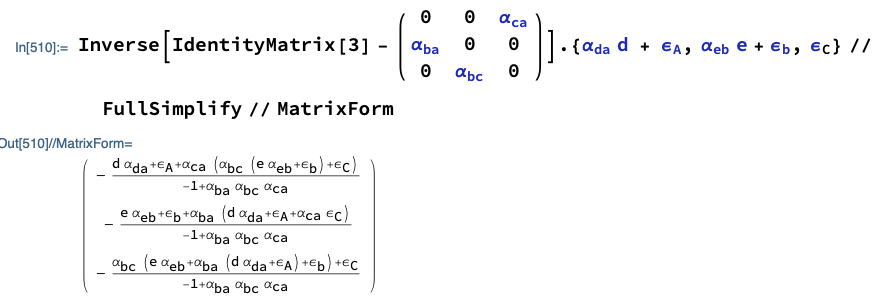
\includegraphics[width=\textwidth]{sol-hw10-2-1.png}}
		\end{figure}
	In the SCM, we replace the equations for $\{A,B,C\}$ with this solution.
	\end{gradedsolution}
	\item Give the graphs $G(\C M)$ and $G(\C M^{\text{acy}})$. (1pt)
	\begin{gradedsolution}
	\begin{tikzpicture}[scale=1, transform shape]
		\tikzstyle{every node} = [draw,shape=circle];
		\node (A) at (0, 0) {$A$};
		\node (B) at (2, 0) {$B$};
		\node (C) at (1, -2) {$C$};
		\node (D) at (-2, 2) {$D$};
		\node (E) at (4, 2) {$E$};
		\node (F) at (1, -4) {$F$};
		\node (epsA) at (-2, 0) {$\epsilon_A$};
		\node (epsB) at (4, 0) {$\epsilon_B$};
		\node (epsC) at (3, -2) {$\epsilon_C$};
		\node (epsD) at (-4, 2) {$\epsilon_D$};
		\node (epsE) at (6, 2) {$\epsilon_E$};
		\node (epsF) at (3, -4) {$\epsilon_F$};
		\draw[-{Latex[length=3mm, width=2mm]}] (epsA) to (A);
		\draw[-{Latex[length=3mm, width=2mm]}] (epsB) to (B);
		\draw[-{Latex[length=3mm, width=2mm]}] (epsC) to (C);
		\draw[-{Latex[length=3mm, width=2mm]}] (epsD) to (D);
		\draw[-{Latex[length=3mm, width=2mm]}] (epsE) to (E);
		\draw[-{Latex[length=3mm, width=2mm]}] (epsF) to (F);
		\draw[-{Latex[length=3mm, width=2mm]}] (D) to (A);
		\draw[-{Latex[length=3mm, width=2mm]}] (E) to (B);
		\draw[-{Latex[length=3mm, width=2mm]}] (A) to (B);
		\draw[-{Latex[length=3mm, width=2mm]}] (B) to (C);
		\draw[-{Latex[length=3mm, width=2mm]}] (C) to (A);
		\draw[-{Latex[length=3mm, width=2mm]}] (C) to (F);
	\end{tikzpicture}
	\begin{tikzpicture}[scale=1, transform shape]
		\tikzstyle{every node} = [draw,shape=circle];
		\node (A) at (0, 0) {$A$};
		\node (B) at (2, 0) {$B$};
		\node (C) at (1, -2) {$C$};
		\node (D) at (-2, 2) {$D$};
		\node (E) at (4, 2) {$E$};
		\node (F) at (1, -4) {$F$};
		\node (epsA) at (-2, 0) {$\epsilon_A$};
		\node (epsB) at (4, 0) {$\epsilon_B$};
		\node (epsC) at (3, -2) {$\epsilon_C$};
		\node (epsD) at (-4, 2) {$\epsilon_D$};
		\node (epsE) at (6, 2) {$\epsilon_E$};
		\node (epsF) at (3, -4) {$\epsilon_F$};
		\draw[-{Latex[length=3mm, width=2mm]}] (epsA) to (A);
		\draw[-{Latex[length=3mm, width=2mm]}, bend left] (epsA) to (B);
		\draw[-{Latex[length=3mm, width=2mm]}] (epsA) to (C);
		\draw[-{Latex[length=3mm, width=2mm]}, bend left] (epsB) to (A);
		\draw[-{Latex[length=3mm, width=2mm]}] (epsB) to (B);
		\draw[-{Latex[length=3mm, width=2mm]}] (epsB) to (C);
		\draw[-{Latex[length=3mm, width=2mm]}] (epsC) to (A);
		\draw[-{Latex[length=3mm, width=2mm]}] (epsC) to (B);
		\draw[-{Latex[length=3mm, width=2mm]}] (epsC) to (C);
		\draw[-{Latex[length=3mm, width=2mm]}] (epsD) to (D);
		\draw[-{Latex[length=3mm, width=2mm]}] (epsE) to (E);
		\draw[-{Latex[length=3mm, width=2mm]}] (epsF) to (F);
		\draw[-{Latex[length=3mm, width=2mm]}] (D) to (A);
		\draw[-{Latex[length=3mm, width=2mm]}] (D) to (B);
		\draw[-{Latex[length=3mm, width=2mm]}] (D) to (C);
		\draw[-{Latex[length=3mm, width=2mm]}] (E) to (B);
		\draw[-{Latex[length=3mm, width=2mm]}] (E) to (A);
		\draw[-{Latex[length=3mm, width=2mm]}] (E) to (C);
		\draw[-{Latex[length=3mm, width=2mm]}] (C) to (F);
	\end{tikzpicture}
		
	\end{gradedsolution}
	\item Show that $\C M^{\text{acy}}$ is observationally equivalent to $\C M$. (1pt)
	\begin{gradedsolution}
		Trivial.
	\end{gradedsolution}
	\item Show that $\C M^{\text{acy}}$ is not interventionally equivalent to $\C M$. (1pt)
	\begin{gradedsolution}
		E.g. intervene $A=a$. Then in $\C M$, $B$ is affected by $a$, but in $\C M^{\text{acy}}$, it is not.
		
	\end{gradedsolution}
	\item Show the following: ($3 \times 1/3$ pts)
	\begin{enumerate}
		\item $D \perp_{G(\C M)}^\sigma F \mid B \iff D \perp_{G(\C M^{\text{acy}})}^d F \mid B$
		\item $D \perp_{G(\C M)}^\sigma E \mid A \iff D \perp_{G(\C M^{\text{acy}})}^d E \mid A$
		\item $D \perp_{G(\C M)}^\sigma E \iff D \perp_{G(\C M^{\text{acy}})}^d E$
	\end{enumerate}
	Note: $\iff$ here means that left and right hand side are either both true or both false.
	\begin{gradedsolution}
		The first two are false. The third is true.

	\end{gradedsolution}
\end{enumerate}

\section{Damped Coupled Harmonic Oscillator: cycles, but simple}
We will prove that the SCM $\C M$ of the equilibrium behaviour of a damped coupled harmonic oscillator in examples 8.11.1 in the lecture notes is simple in the following steps.

\begin{enumerate}
\item Preliminary (1pt):
\begin{enumerate}
	\item Prove that for any\footnote{It's more straightforward to see this in the general case.} SCM satisfying the assumptions of proposition 8.1.3 that invertibility of $1_{V}-B_{VV}$ ensures that the SCM has a unique solution.
\end{enumerate}

\item Steps for SCM $\C M$ ($3 \times 1$ pt):
\begin{enumerate}
	\item Show that $\C M$ satisfies the assumptions of proposition 8.1.3 in the lecture notes.
	\item Write the matrix $1_{V}-B_{VV}$ (where $1_V$ is the $|V|\times |V|$ identity matrix) as a tridiagonal matrix (\url{https://en.wikipedia.org/wiki/Tridiagonal_matrix}) and show that the determinant is non-zero and thus the matrix invertible.

	Hint: you can use that the determinant of a tridiagonal matrix of the following
form is given by the expression on the r.h.s.\footnote{Bonus point for who comes up with an elegant proof of this identity that does not rely on solving the recurrence relationship for the determinant of tridiagonal matrices.}:
  $$\det \begin{pmatrix}
    k_0+k_1 & -k_1       &           &         & \\
    -k_1     & k_1 + k_2 & -k_2       &         & \\
            & -k_2       & k_2 + k_3 & \ddots  & \\
            &           & \ddots    & \ddots  & -k_{d-1} \\
            &           &           & -k_{d-1} & k_{d-1} + k_d \\
  \end{pmatrix} = \sum_{i=0}^d \prod_{j=0 \atop j\ne i}^d k_j
  $$
  In order to obtain the above form, factorize the matrix $1_{V}-B_{VV}=MN$, where $N$ is of the above form and $M$ is diagonal. Use $\det MN=\det M \det N$.
	\item For for any $T \subseteq V$, the matrix $1_{V \setminus T}-B_{(V \setminus T)(V \setminus T)}$ is also invertible and thus that the SCM is simple. You can use the fact that the determinant of a block-diagonal matrix is the product of the determinant of the constituent matrices.
\end{enumerate}
\end{enumerate}
\begin{gradedsolution}
	\begin{align*}
		&1_V-B_{VV}\\
		&=\begin{pmatrix}
			1 & -k_1/(k_1+k_0) & 0 & 0 & ... \\
			-k_1 / (k_2+k_1) & 1 & -k_2 / (k_2+k_1) & 0 & ... \\
			0& -k_2 / (k_3+k_2) & 1 & -k_3 / (k_3+k_2) & ... \\
			... & ... & ... & ... & ... 
		\end{pmatrix}\\
		&=\begin{pmatrix}
			1/(k_1+k_0) & 0 & 0 & 0 & ... \\
			0& 1/ (k_2+k_1) &  & 0 & ... \\
			0& 0& 1 / (k_3+k_2) &0& ... \\
			... & ... & ... & ... & ... 
		\end{pmatrix}
		\begin{pmatrix}
			k_0+k_1 & -k_1       &     0     &    \dots     \\
			-k_1     & k_1 + k_2 & -k_2       &  \dots        \\
			0		& -k_2       & k_2 + k_3 &  \dots \\
				\dots	&   \dots        & \dots   & \dots  
		  \end{pmatrix}
	\end{align*}
	The determinant of the first matrix is the product of the diagonals, the second is the given by the hint. Both are clearly positive for positive $k_i>0$.

	For any intervention, just look at the unintervened connected components, compute the determinant and multiply. This will also be positive.

	In general, if $x=Ax+b$ and $(1-A)$ is invertible, then $x=(1-A)^{-1}b$ is the unique solution.
\end{gradedsolution}

\section{Price, supply and demand: self-cycles and still uniquely solvable, but not simple}
Consider the dynamical system and the SCM given in Example 8.11.3 of the lecture notes.
\begin{enumerate}
	\item Show for which of the 8 subsets $T \subseteq \{S, R, D\}$, the intervened SCM $\C M_{\text{do}(T)}$ is uniquely solvable. You can use the condition for unique solvability of linear SCMs from example 8.1.3 of the lecture notes. (1pt)
	\item For all possible interventions $T \subseteq \{S, R, D\}$, show whether the dynamical has an equilibrium and if it exists compute this equilibrium. (1pt)
\end{enumerate}
We see that when the intervened SCM is uniquely solvable, its solution indeed equals the equilibrium of the intervened dynamical system.
\begin{gradedsolution}
\begin{enumerate}
	\item We have a linear system with matrix (in order D,S,R): $1_3 - \begin{pmatrix}0 & 0 & \beta_D \\ 0 & 0 & \beta_S \\ 1 & -1 & 1\end{pmatrix}$. Taking the determinant for any subset of rows/cols, assuming $\beta_S-\beta_D>0$, we find zero determinant only if $T=\{D, S\}$. In only this case, no unique solutions exists.
	\item If $T=\{D, S\}$, then $R$ diverges (unless when $D-S=0$, when any $R$ is a solution).
\end{enumerate}
\end{gradedsolution}

\end{document}
